\documentclass[11pt]{article}
\usepackage[utf8x]{inputenc}
\usepackage{graphicx}
\usepackage{natbib}
\usepackage[left=1in, right=1in, top=1in, bottom=1in]{geometry}
\usepackage{titling}


\pretitle{\begin{center}\Huge\bfseries}
\posttitle{\par\end{center}\vskip 0.5em}
\preauthor{\begin{center}\Large\ttfamily}
\postauthor{\end{center}}
\predate{\par\large\centering}
\postdate{\par}

\title{SVHN: Machine Learning and Practical Image Recognition}
\author{Sajith Kumar (svaz0513), Sahar Nourazar (snou3270), James Macdonald (jmac7228)}
\date{\today}
\begin{document}

\maketitle
\thispagestyle{empty}

\begin{abstract}
This paper compares the performance of different machine learning algorithms on the Street View House Numbers dataset. This paper examines Support Vector Machines, Random Forest, and Neural Network methods, evaluating performance across a number of metrics.
\end{abstract}

\section{Introduction}
 
Machine learning has demonstrated reliable, accurate performance in image recognition tasks. On datasets such as MNIST, simple neural networks can achieve over 99\% accuracy \citep{tfmnist}. High performance is being achieved in other, more practical problems. The Street View House Numbers dataset (SVHN) is a series of labelled images depicting house numbers taken from google images. The dataset has been cropped to centre the relevant number in a 1024 pixel square image. The training set comprises 73,257 and the validation set contains a further 26,032 images. Training is conducted via cross-validation, but performance is determined by the accuracy achieved both on the kfold hold-out and the separate, hold-out validation set. Supplementary metrics will be similarly explored in further analysis.\\

The purpose of this study is twofold: firstly, to compare the performance of newer, specialist methods of image classification against that of more generalist algorithms. The generalist algorithms used are Support Vector Machines (SVM) and Random Forest (RF), and are 'generalist' in the sense that they have no special image recognition preprocessing. The specialist method is a Convolutional Neural Network (CNN), with two permutations. The first involves 'vanilla' CNN that stacks convolutional layers and fully-connected layers. The second permutation first uses a K-means clustering implementation to construct features, and feeds those features to a CNN for enhanced performance. This study will investigate the performance uplift of specialist methods over generalist methods.\\

The second purpose of this study is to investigate the 'accessibility' of top-of-the-range performance. The highest-scoring algorithms can achieve over 98\% out-of-sample accuracy. This study investigates how achievable those results for masters-level students with standard tooling and resources. For neural networks, this means a readily available solution like Tensorflow or Keras. For other classifiers, this means it must be available in the python data science library Scikit-Learn. Any preprocessing was done either using these or lower-level libraries, such as numpy.\\

This study is important because it draws a link between the cutting edge of machine learning techniques and mainstream implementations. It is important to democratize and propagate breakthroughs in academic research, and this study examines how far behind mainstream implementations lie.

\section{Methodology}

\subsection{The Problem}
The SVHN problem is similar to MNIST, in that the goal is to identify digits in images. However, the SVHN data adds a number of layers of complexity to the problem not present in MNIST. For one, SVHN contains data from real-world images, so there are complications such as lighting, angle, and possible obstruction. Secondly, a given SVHN data may contain multiple numbers in a single frame, and the classifier must identify which ones are noise, and which ones are the label.\\

There is an additional, optional layer of difficulty in this problem. The SVHN data is presented in two forms, firstly the raw, unzoomed snapshots from Google Street View, secondly a tightly cropped set of 32x32 images that centre the relevant number. The first form of the data is a much trickier problem in that a classifier must first preprocess the image to detect an unknown number of numbers with unknown positions. This additional layer will not be looked at in the model comparison, but touched on in further analysis.

\subsection{Data Preprocessing}
As outlined in the introduction, this study compares 2 main types of approaches: generalist methods and specialist methods.\\

Firstly, the data is converted to greyscale. This significantly reduces the dimensionality of the data and thus makes training much faster. Colour plays no part in determining a number, so the conversion should not remove any useful information. The conversion to greyscale is done line with human sight, so channels are not uniformly weighted. Exact weights are given in the code.
\begin{figure}[h]
\caption{The effect of preprocessing the data from colour to greyscale}
\centering
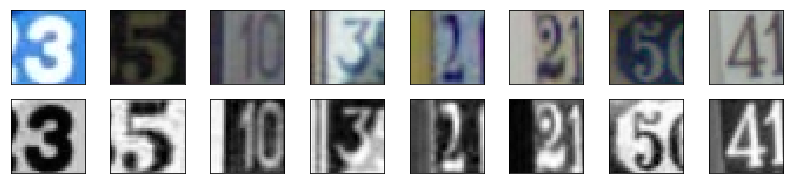
\includegraphics[width=0.9\textwidth]{images/colour_to_greyscale.png}
\end{figure}

Secondly, the data is run through a Principle Component Analysis (PCA). Reducing the dimensionality again allows for much faster training of the algorithm. However, since convolutional steps require the concept of the image in order to extract features, PCA was only done for generalist solutions.
\begin{figure}[h]
\caption{Information retained by taking the N largest eigenvalues}
\centering
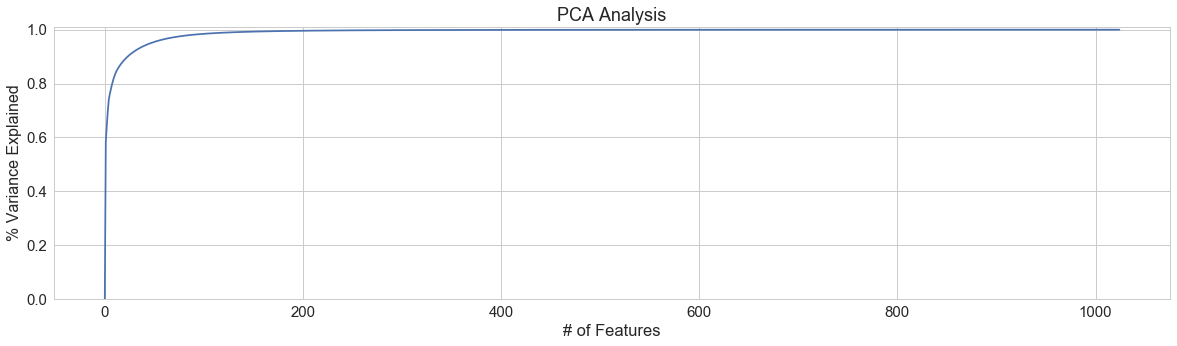
\includegraphics[width=0.9\textwidth]{images/pca_information_retention.png}
\end{figure}

\subsection{Generalist Solutions: Support Vector Machines}
The first classification approach used an SVM classifier on preprocessed data. Scikit-learn offers an out-of-the-box SVM classification tool, called SVC. There is some hyper-parameter tuning involved in fitting an SVC. For kernel selection, Gaussian methods outperform other variations for image classification\citep{svmkernels}, and for this reason the Gaussian Radial Basis Function (RBF) was selected. A Randomized Search was conducted on a 5000-row sample of the data to select the regularization parameter C, and the kernel coefficient gamma. Randomized search was chosen because it retains many benefits of Grid Search (simplicity in concept and implementation) while having high efficiency in high-dimensional search spaces.\\

After hyperparameter tuning, the algorithm was trained via k-fold cross validation with 10 folds. The holdout sets were scored, and those scores were combined to create the final scored dataset. Unfortunately, SVM solutions do not neatly return the probabilities that each observation belongs to a given class. Scikit-learn's solution offers a heuristic


\subsection{Generalist Solutions: Random Forest}
The second classification approach used a Random Forest (RF) algorithm. RF models are an ensemble of decision trees, which separate the data by splitting on features which best segment out distinct classes. Each tree being exposed to a subset of features. This structure means that the model automatically regularizes well, since no tree has the opportunity to learn the data. \\

RF models have some hyperparameters that require tuning, namely max tree depth and total number of trees. These were tuned on a small, 2000-row sample of the data. Once optimal values of hyperparameters were determined, the algorithm was trained via 10-fold cross validation, with hold-out sets combined into the results dataset.

\subsection{Specialist Solutions: Convolution Neural Network}
The final classification approach was a Convolutional Neural Network (CNN), a machine-learning algorithm adapted specifically for image classification tasks. CNNs consist of a number of trainable layers that fall into the following categories:
\begin{itemize}
  \item Convolutional layers: 2-dimensional filters applied to a subset of pixels that multiply the pixel fill by trainable weights
  \item Pooling layers: 2-dimensional filters that apply an operation over a subest of pixels, usually to extract the maximum value (a process known as maxpooling)
  \item Fully-Connected layers: A 1-dimensional array of trainable weights that multiply input features, and then apply a non-linear activation function (such as Rectified Linear Units)
\end{itemize}

There are two important attributes of CNNs that suit image recognition data. The first is the previously mentioned specialized layers (convolutional and pooling). Also, image data represents high-dimensional space. The training algorithms of neural networks scale much better than techniques like SVM, both in terms of dimensionality and number of observations.

In order to generalise the solution, both drop-out and l2 regularization techniques were employed. Drop-out prevents the network from leaning too heavily on individual nodes by assigning each node a probability that its output will be set to zero. L2 regularization applies a penalty to the magnitude of weights, encouraging the network to use smaller coefficients and thus inhibiting overfitting.

The full set of hyperparameters to be tuned in the neural network is:
\begin{itemize}
\item Batch size
\item Network architecture (including number of layers, type of layer, filters/neurons per layer)
\item Dropout
\item L2 regularization
\item Learning rate
\item Number of iterations
\end{itemize}

These were all adjusted manually by observing network performance on out-of-sample data as hyperparameters were tweaked. After tuning, a K-fold cross validation was performed on the training dataset. Performance on the holdout set is explored in the results section. The in-sample performance was tracked to see the performance of the AdamOptimizer algorithm. This is shown below:

\begin{figure}[h]
\caption{CNN in-sample performance by iteration (the average is given in black)}
\centering
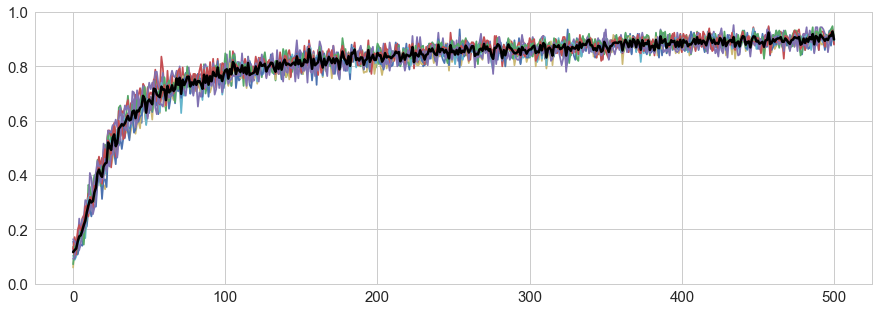
\includegraphics[width=0.9\textwidth]{images/training-progress.png}
\end{figure}
 
\medskip
 
% To change the title from References to Bibliography:
\renewcommand\refname{Bibliography}

\bibliographystyle{unsrtnat} % or try abbrvnat or unsrtnat
\bibliography{references} % refers to example.bib
 
\end{document}
